\begin{document}
\maketitle

\begin{abstract}
From the admissible reduced datum
\[
\Tmin^{\mathrm{adm}}=(\mathcal A,\mathcal H,D,J,\Gamma,\inv,\nu),
\]
the carrier-first architecture reconstructs the primitive layer, the unique minimal carrier
$E_3\oplus E_2$, the global Standard Model quotient
$S(U(3)\times U(2))\cong(SU(3)\times SU(2)\times U(1)_Y)/\mathbb Z_6$, one chiral family
with $\nu^c$ from the positive half-spinor, the hypercharge--seam inversion
$6Y^2-Y-\mathbf 1=0$, and the exact electromagnetic closure equation whose canonical
admissible branch reproduces $\alpha^{-1}(0)=\num{137.0359992}$.

The same theorem surface then generates the canonical two-stage admissibility selector
\[
\Padm=P_{\mathrm{str}}P_{\mathrm{gap}},
\qquad
P_{\mathrm{str}}:=P_{\Seam,+}P_{\mathrm{sing}}P_\Theta,
\]
the topological family closure $F\cong\mathbb C^3$ and $\Oadm=48$, and a conditional
geometric reconstruction in which the Dirac anchor
\[
D_{\mathrm{geo}}:=D_{\mathrm{ref}}+D_{\mathrm{rel}}=D
\]
carries the metric, spin, and local spectral-scale data while the admissible compression
governs retained observables. The transport sector is organized on a canonical numerically
selected admissible branch with exact Yukawa formulas, hadronic singlet selection,
strong-CP protection, reflection positivity, and Lorentzian reconstruction.

The observation layer is formulated as a conditional closure selection theorem: once
coercivity and local Hessian positivity hold on the admissible domain, selected minimizers
are read by the observation functor $\mathcal R_{\mathrm{TOE}}$. Matched benchmark ledgers
are reported on the canonical selected branch, while optional downstream modules evaluate
UV Bernstein-cone and cosmology-facing quantities from the same retained operator data.

Compression identities remain structural rather than decorative: once the optional occupancy
compression is imposed, the rank-lock $2^{g-3}=g-1$ fixes $g=5$, the hard $41$-chain
$10\,b_1=\Omega_{\mathrm{adm}}\gamma+1=41$ overdetermines the canonical branch, and wrong
discrete worlds still fail the electromagnetic closure decisively. Optional E$_8$
arithmetic continuations, asymptotic expansions, and horizon language are retained only as
appendix-level extrapolations and are not part of the closed theorem surface.
\end{abstract}

\begin{tcolorbox}[colback=tfptblue!2, colframe=tfptblue!40, breakable,
    title={Reading Status for the Present Paper}, colbacktitle=tfptblue!60]
\begin{itemize}[leftmargin=1.5em, topsep=3pt, itemsep=3pt]
    \item \textbf{Reduced datum:} $\Tmin^{\mathrm{adm}}=(\mathcal A,\mathcal H,D,J,\Gamma,\inv,\nu)$ with admissible spectral regularity, seam collar, and positive spectral measure.
    \item \textbf{Status classes:} exact algebraic, conditional geometric or closure, matched intrinsic observation, and optional extrapolation.
    \item \textbf{Exact algebraic layer:} primitive scaffold, minimal carrier $E_3\oplus E_2$, one-family packet, carrier constants, and exact electromagnetic closure.
    \item \textbf{Conditional geometric or closure layer:} two-stage admissibility selector, topological family closure, Dirac-anchor geometry, transport-branch program, hadronic and strong-CP closure, Lorentz reconstruction, and the conditional UV Bernstein-cone program.
    \item \textbf{Matched intrinsic observation layer:} selected-branch ledgers, threshold rows, and the observation functor $\mathcal R_{\mathrm{TOE}}$.
    \item \textbf{Optional downstream modules:} cosmology-facing evaluations, E$_8$ scale grammar, asymptotic expansions, and horizon semantics.
\end{itemize}
\end{tcolorbox}

\tableofcontents

\section{Reading guide and claim map}

The paper is organized in three reading layers:
\begin{itemize}[leftmargin=1.5em, topsep=3pt, itemsep=2pt]
    \item \textbf{Big picture:} one section explains what TFPT claims in plain language before the detailed datum and conventions begin.
    \item \textbf{Detail:} the main body then runs from primitive core and hard carrier kernel through kernel numerics, the two closure-architecture sections, the closure theorem stack, the particle/mass compiler, and the benchmark interface.
    \item \textbf{Proof sketches:} the main text gives only the central proof sketches, while dense technical derivations remain in appendices or companion material.
\end{itemize}
The status language is also fixed once and for all:
\begin{itemize}[leftmargin=1.5em, topsep=3pt, itemsep=2pt]
    \item \textbf{Reduced datum} means the admissible spectral starting package from which the primitive scaffold is reconstructed.
    \item \textbf{Exact algebraic} means exact consequences of the carrier algebra, parity code, weight enumerator, and compression identities.
    \item \textbf{Conditional geometric or closure} means statements that depend on the geometric anchor, admissibility closure, APS input, positivity input, or selected retained branch.
    \item \textbf{Matched intrinsic observation} means rows read through the observation functor and benchmark map, including threshold outputs and convention-dependent comparisons.
    \item \textbf{Optional extrapolation} means appendix-level continuations not needed for the core.
\end{itemize}
To keep theorem language, benchmark semantics, and appendix bookkeeping lexically stable, all prose, captions, and status labels are kept in English throughout.

\begin{tcolorbox}[colback=tfptblue!2, colframe=tfptblue!40, breakable,
    title={Datum Hierarchy for the Present Draft}, colbacktitle=tfptblue!60]
\begin{itemize}[leftmargin=1.5em, topsep=3pt, itemsep=3pt]
    \item \textbf{Reduced datum:} $\Tmin^{\mathrm{adm}}$ with admissible center, involution, seam collar, and positive spectral measure.
    \item \textbf{Exact algebraic layer:} reconstructed primitive scaffold, minimal carrier $E_3\oplus E_2$, global quotient, one-family packet, and exact electromagnetic closure.
    \item \textbf{Conditional geometric or closure layer:} $\Padm$, topological family closure, Dirac-anchor geometry, Higgs selection, transport-branch program, hadronic sector, and conditional UV closure.
    \item \textbf{Matched intrinsic observation layer:} selected-branch thresholds, ledgers, and observable generation through $\mathcal R_{\mathrm{TOE}}$.
    \item \textbf{Optional extrapolation:} cosmology-facing modules, E$_8$ continuations, asymptotic transport expansions, and horizon semantics.
\end{itemize}
\end{tcolorbox}

\begin{figure}[t]
\centering
\begin{tikzpicture}[
    scale=0.58,
    transform shape,
    >=Latex,
    node distance=1.6cm and 1.7cm,
    primitive/.style={draw=gray!70!black, thick, rounded corners, fill=gray!10, align=center, minimum width=2.8cm, minimum height=1cm},
    hard/.style={draw=blue!60!black, thick, rounded corners, fill=blue!4, align=center, minimum width=2.8cm, minimum height=1cm},
    bridge/.style={draw=green!50!black, dashed, thick, rounded corners, fill=green!4, align=center, minimum width=2.9cm, minimum height=1cm},
    closure/.style={draw=orange!70!black, dotted, thick, rounded corners, fill=orange!5, align=center, minimum width=3.0cm, minimum height=1cm},
    optional/.style={draw=purple!70!black, dash pattern=on 4pt off 2pt on 1pt off 2pt, thick, rounded corners, fill=purple!5, align=center, minimum width=3.0cm, minimum height=1cm}
]
\node[primitive] (core) {$\Tprim$\\primitive datum and spectral seed};
\node[hard, right=of core] (carrier) {$\Tker$\\carrier packet and one family};
\node[closure, right=of carrier] (bridge) {$\Padm$, $F$, $\Oadm$\\closure selector and family theorem};
\node[closure, below=of carrier] (geom) {$\Ageom$\\Higgs, $\sigma/\chigeo$, superconnection};
\node[closure, below=of bridge] (trans) {$\Atrans$\\Yukawas, confinement, strong CP};
\node[bridge, right=of bridge] (cmp) {matched intrinsic observation\\$\mathcal R_{\mathrm{TOE}}$, ledgers, observation images};
\node[optional, below=of cmp] (cond) {optional layer\\E$_8$ and horizons};
\draw[->, thick] (core) -- (carrier);
\draw[->, thick] (carrier) -- (bridge);
\draw[->, dotted, thick] (carrier) -- (geom);
\draw[->, dotted, thick] (bridge) -- (trans);
\draw[->, dashed, thick] (bridge) -- (cmp);
\draw[->, dotted, thick] (geom) -- (cmp);
\draw[->, dotted, thick] (trans) -- (cmp);
\draw[->, dash pattern=on 4pt off 2pt on 1pt off 2pt, thick] (cmp) -- (cond);
\coordinate (legone) at ($(geom.south west)+(-0.9,-2.3)$);
\draw[->, thick, gray!70!black] (legone) -- ++(1.2,0) node[right, black, font=\scriptsize] {Reduced datum};
\coordinate (legtwo) at ($(legone)+(0,-0.6)$);
\draw[->, thick] (legtwo) -- ++(1.2,0) node[right, black, font=\scriptsize] {Exact algebraic};
\coordinate (legthree) at ($(legtwo)+(0,-0.6)$);
\draw[->, dotted, thick] (legthree) -- ++(1.2,0) node[right, black, font=\scriptsize] {Conditional closure};
\coordinate (legfour) at ($(legthree)+(0,-0.6)$);
\draw[->, dashed, thick] (legfour) -- ++(1.2,0) node[right, black, font=\scriptsize] {Matched intrinsic observation};
\coordinate (legfive) at ($(legfour)+(0,-0.6)$);
\draw[->, dash pattern=on 4pt off 2pt on 1pt off 2pt, thick, purple!70!black] (legfive) -- ++(1.2,0) node[right, black, font=\scriptsize] {Optional extrapolation};
\end{tikzpicture}
\caption{Claim map for the carrier-first compiler form across reduced datum, exact algebraic outputs, conditional closure statements, matched intrinsic observation rows, and optional extrapolations.}
\label{fig:dependency-map}
\end{figure}

\begin{table}[t]
\centering
\scriptsize
\begin{tabularx}{\linewidth}{@{}>{\raggedright\arraybackslash}p{0.23\linewidth}>{\raggedright\arraybackslash}p{0.12\linewidth}YY@{}}
\toprule
Layer or statement & Role & Proof source or remaining note & Main empirical or structural test \\
\midrule
Admissible reduced datum and Bernstein spectral action & Reduced datum & admissible datum definition and primitive reconstruction theorem in the main text & failure would collapse the operator-level starting point \\
Oriented double cover, seam, involution & Exact algebraic & primitive kinematic scaffold theorem in the main text & structural consistency of all later layers \\
Minimal carrier $E_3\oplus E_2$ & Exact algebraic & proof sketch given in \Cref{sec:minimal-carrier-proof} & failure would collapse the whole packet \\
One-family packet $S^+=\Lambda^{\mathrm{even}}E$ & Exact algebraic & decomposition and proof sketch given in the main text & group/matter mismatch would be global \\
Carrier coefficient function $\bone(N_{\mathrm{fam}},N_\Phi)$ & Exact algebraic & abelian-index formula in the main text & hypercharge-trace mismatch would be structural \\
Canonical seam/kernel constants $(\cthree,\phibase,\deltatop)$ & Exact algebraic & seam normalization, exact seam opening, and carrier-form closure equations summarized in the main text & scheme discipline for observable comparison \\
Canonical closure value $\bone=41/10$ & Exact algebraic & canonical family/Higgs closure of the abelian index on the admissible branch & failure would break the 41-chain and the canonical packet count \\
Operative admissibility selector $\Padm$ & Conditional geometric or closure & two-stage admissibility complex in \Cref{sec:closure-theorems} & unified electroweak / QCD / CP sector selection \\
Family closure, $F\cong\mathbb C^3$, and $\Oadm=48$ & Conditional geometric or closure & topological family closure and occupancy corollary in \Cref{sec:closure-theorems} & flavor multiplicity and family lifting \\
Bosonic relative index selecting $\Phi$ & Conditional geometric or closure & Callias Higgs-selection theorem and bosonic closure theorem in \Cref{sec:closure-theorems} & unique light doublet / doublet-triplet split \\
Local spectral-scale / gravity closure for $\Mpl$ and $\vgeo$ & Conditional geometric or closure & Dirac-anchor geometry, bosonic closure, and two-sheet zero-mode lemma & Planck / electroweak / gravity relation \\
Yukawa holonomy matrix and mass closure & Conditional geometric or closure & transport-branch program and exact family-holonomy phase control & $m_f$, CKM / PMNS, hierarchy grammar \\
Hadronic space, anomaly inflow, and strong CP & Conditional geometric or closure & hadronic / anomaly closure theorems in \Cref{sec:closure-theorems} & hadron spectrum and $\bar\theta$ null tests \\
Nonperturbative QFT closure & Conditional geometric or closure & gap lift, Callias positivity bounds, and admissible QFT theorem & mass gap, clustering, and confinement route \\
Reflection positivity, Lorentz reconstruction, record algebra, and vacuum closure & Conditional geometric or closure & relative generating functional, admissible reflection-positivity lemma, gap/clustering record construction, split OS / vacuum theorems, and primitive Lorentzian corollary & causal dynamics, stable records, and vacuum energy map \\
Observation functor $\mathcal R_{\mathrm{TOE}}$, threshold outputs, and benchmark rows & Matched intrinsic observation & conditional closure-selection theorem with scheme-covariant numerical preconditioner $\mathcal R_{\SM}$ & convention-complete theory-versus-data translation \\
E$_8$ and horizon semantics & Optional extrapolation & deferred to appendices and the auxiliary appendix continuation & downstream extension rather than main-text hard claim \\
\bottomrule
\end{tabularx}
\caption{Status matrix for the carrier-first compiler form with reduced datum, exact algebraic outputs, conditional closure statements, matched intrinsic observation rows, and optional extrapolations kept visibly distinct.}
\label{tab:status-matrix}
\end{table}

The family closure used throughout the main text is now read as topologically fixed and
canonically compatible with the doubled admissible branch; no separate family datum remains
outside the theorem surface.

\section{Big picture: what TFPT actually claims}

TFPT is presented here as a carrier-first theory of admissible vacua on the oriented double cover. The primitive datum fixes the relative spectral starting package before any carrier decomposition is imposed. The hard carrier theorem then enforces the minimal split $E_3\oplus E_2$ and hence the global Standard Model group, hypercharge, one chiral family, seam normalization, and the carrier-form electromagnetic closure equation. Under the declared admissibility, $\APSdom$, Bernstein-kernel positivity, and reflection-positivity axioms, the same architecture closes further: the two-stage selector makes $\Padm$ operative, the topological family theorem fixes $F$ and $N_{\mathrm{fam}}=3$, the Callias index selects the Higgs, the Dirac anchor carries the geometric reconstruction, and the discrete transport grammar emits Yukawas and mixings on a canonical numerically selected branch. Hadronic singlet selection, strong-CP protection, Lorentz reconstruction, and the admissible vacuum remain on that main-text surface, while UV and cosmology-facing continuations are stated explicitly as conditional or downstream modules. The comparison map then translates the selected compiler surface into PDG-style observables.

\Cref{fig:tfpt-headline-claims} compresses that statement into six headline claims. The point is
not that every downstream extension is already proved without qualification, but that the present
draft claims a small carrier-first kernel with unusually broad structural reach.

\begin{figure}[t]
\centering
\scriptsize
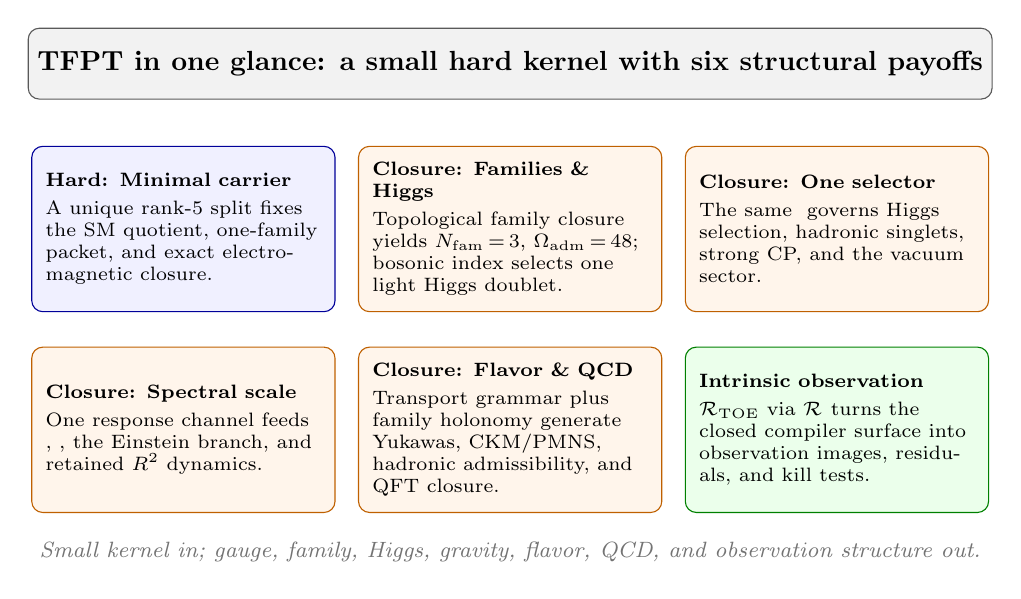
\begin{tikzpicture}[
    headline/.style={draw=black!65, fill=gray!10, rounded corners, minimum width=11.6cm, minimum height=0.9cm, align=center, font=\bfseries},
    hard/.style={draw=blue!60!black, fill=blue!6, rounded corners, text width=3.5cm, minimum height=2.1cm, align=left, inner sep=5pt, font=\scriptsize},
    closure/.style={draw=orange!75!black, fill=orange!8, rounded corners, text width=3.5cm, minimum height=2.1cm, align=left, inner sep=5pt, font=\scriptsize},
    bridge/.style={draw=green!50!black, fill=green!8, rounded corners, text width=3.5cm, minimum height=2.1cm, align=left, inner sep=5pt, font=\scriptsize},
    note/.style={font=\footnotesize\itshape, text=black!55, align=center}
]
\node[headline] (head) at (0,0) {TFPT in one glance: a small hard kernel with six structural payoffs};

\node[hard] (a) at (-4.15,-2.1) {\textbf{Hard: Minimal carrier}\\[2pt]A unique rank-$5$ split fixes the SM quotient, one-family packet, and exact electromagnetic closure.};
\node[closure] (b) at (0,-2.1) {\textbf{Closure: Families \& Higgs}\\[2pt]Topological family closure yields $N_{\mathrm{fam}}\!=\!3$, $\Omega_{\mathrm{adm}}\!=\!48$; bosonic index selects one light Higgs doublet.};
\node[closure] (c) at (4.15,-2.1) {\textbf{Closure: One selector}\\[2pt]The same $\Padm$ governs Higgs selection, hadronic singlets, strong~CP, and the vacuum sector.};

\node[closure] (d) at (-4.15,-4.65) {\textbf{Closure: Spectral scale}\\[2pt]One response channel feeds $\Mpl$, $\vgeo$, the Einstein branch, and retained $R^2$ dynamics.};
\node[closure] (e) at (0,-4.65) {\textbf{Closure: Flavor \& QCD}\\[2pt]Transport grammar plus family holonomy generate Yukawas, CKM/PMNS, hadronic admissibility, and QFT closure.};
\node[bridge] (f) at (4.15,-4.65) {\textbf{Intrinsic observation}\\[2pt]$\mathcal R_{\mathrm{TOE}}$ via $\mathcal R_{\SM}$ turns the closed compiler surface into observation images, residuals, and kill tests.};

\node[note] at (0,-6.2) {Small kernel in; gauge, family, Higgs, gravity, flavor, QCD, and observation structure out.};
\end{tikzpicture}
\caption{Headline claims of the present draft. The figure is intentionally simpler than the
dependency maps that follow: its job is to put the manuscript's core payoff on one page, while
still keeping the hard / closure / intrinsic-observation split visible.}
\label{fig:tfpt-headline-claims}
\end{figure}

\begin{tcolorbox}[colback=tfptblue!3, colframe=tfptblue, breakable,
    title={TFPT master equation and selectors}, colbacktitle=tfptblue]
\begin{equation}
\label{eq:tfpt-master}
\begin{aligned}
S_{\mathrm{TFPT}}
=
\operatorname{Tr}f\!\left(\frac{D_{\mathrm{rel}}+A_{\Sigma}^{\mathrm{seed}}}{\chiseed}\right)
-
\operatorname{Tr}f\!\left(\frac{D_{\mathrm{ref}}}{\chiseed}\right)
+\frac{i\pi}{2}\Delta\eta_\Sigma,
\qquad
A_{\Sigma}^{\mathrm{seed}}:=\mathcal B_{\mathrm{rel}}\oplus\nabla_{\chiseed}.
\end{aligned}
\end{equation}
\begin{equation}
\label{eq:tfpt-selectors}
\begin{aligned}
\operatorname*{Stat}_{\alpha,\chiseed,e,\wspin}S_{\mathrm{TFPT}}=0,
\qquad
\Padm:=P_{\mathrm{str}}P_{\mathrm{gap}},
\qquad
P_{\mathrm{str}}:=P_{\Seam,+}P_{\mathrm{sing}}P_\Theta,
\\
\operatorname{Ind}_{APS}(D^+_{\mathrm{rel}}\otimes L_F)=3,
\qquad
\operatorname{Ind}^{\Padm}_{\mathrm{rel}}(\mathcal B^+_{E_2})=1,
\qquad
\operatorname{Ind}^{\Padm}_{\mathrm{rel}}(\mathcal B^+_{E_3})=0.
\end{aligned}
\end{equation}
\end{tcolorbox}

The hard carrier theorems below do not require the full closure stack behind
\Cref{eq:tfpt-master,eq:tfpt-selectors}. In the present paper the master equation is the
organizing compiler form, the carrier theorems are hard, and the later closure theorems are
internal statements on the admissible reduced datum rather than extra primitive ontology. At this
overview level the seed package is written as $A_{\Sigma}^{\mathrm{seed}}$; on the later
geometric branch it is reorganized as $A_{\Sigma}^{\mathrm{geo}}$ with
$\chiseed\mapsto\chigeo=\Lambda e^\sigma$.

\begin{tcolorbox}[colback=tfptblue!3, colframe=tfptblue, breakable,
    title={Closed TFPT Chain}, colbacktitle=tfptblue]
\begin{equation}
\label{eq:compiler-chain}
\begin{aligned}
\Tmin^{\mathrm{adm}}
&\Rightarrow
( \Tprim^{\mathrm{kin}},\ E_3\oplus E_2,\ G_{\SM}^{\mathrm{glob}},\ S^+)\\
&\Rightarrow
( \Padm,\ F,\ g,\ \sigma,\ \Phi,\ \nabla_F^\star )\\
&\Rightarrow
x_{\mathrm{core}}^\star
\;\Rightarrow\;
\mathcal R_{\mathrm{TOE}}
\;\Rightarrow\;
(O_{\mathrm{th}},\ \Pred).
\end{aligned}
\end{equation}
\end{tcolorbox}

\begin{tcolorbox}[colback=tfptorange!4, colframe=tfptorange!80!black, breakable,
    title={Closed Theorem Stack in the Present Version}, colbacktitle=tfptorange!85!black]
\begin{gather*}
\Tmin^{\mathrm{adm}}
\;\Rightarrow\;
\Tprim
\;\Rightarrow\;
\text{carrier/kernel}
\;\Rightarrow\;
\text{admissibility + geometry + flavor + vacuum}\\[2pt]
\Rightarrow\;
\text{UV + cosmology}
\;\Rightarrow\;
\mathcal R_{\mathrm{TOE}}
\;\Rightarrow\;
O_{\mathrm{th}}.
\end{gather*}
The main text contains no additional primitive ontology beyond the reduced datum.
Several downstream arrows remain explicitly conditional and are marked as such below.
Optional arithmetic continuations, asymptotic expansions, and horizon language are kept only in appendices.
\end{tcolorbox}

\begin{figure}[t]
\centering
\scriptsize
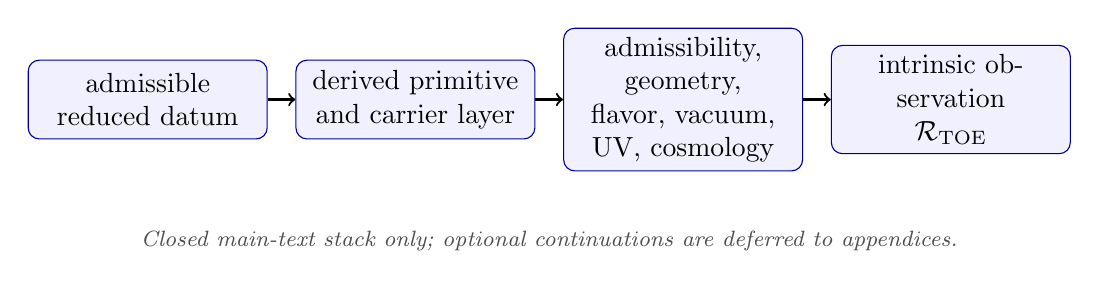
\begin{tikzpicture}[
    closed/.style={draw=blue!60!black, fill=blue!6, rounded corners, text width=2.8cm, minimum height=1.0cm, align=center},
    note/.style={font=\footnotesize\itshape, text=black!70, align=center}
]
\node[closed] (a) at (-5.1,0) {admissible\\reduced datum};
\node[closed] (b) at (-1.7,0) {derived primitive\\and carrier layer};
\node[closed] (c) at (1.7,0) {admissibility, geometry,\\flavor, vacuum, UV, cosmology};
\node[closed] (d) at (5.1,0) {intrinsic observation\\$\mathcal R_{\mathrm{TOE}}$};
\draw[->, thick] (a) -- (b);
\draw[->, thick] (b) -- (c);
\draw[->, thick] (c) -- (d);
\node[note] at (0,-1.8) {Closed main-text stack only; optional continuations are deferred to appendices.};
\end{tikzpicture}
\caption{Closed theorem surface in the present draft. The main text runs from the admissible
reduced datum through the derived closure stack to the intrinsic observation functor, with no
parallel theorem ladder carried in parallel.}
\label{fig:status-ladder}
\end{figure}

The remainder of the main text sharpens each arrow of this chain in turn.

\section{Primitive core and hard carrier kernel}

\subsection{Primitive core and conventions}

We use natural units $c=\hbar=1$. Relative operators are formulated in Euclidean signature and compared through a declared Wick-rotation bridge when Lorentzian language is needed. Higgs fields are denoted by $\Phi$, Hamiltonians by $\mathcal H$, and the cosmological Hubble rate by $\Hhub(t)$; this avoids overloading the letter $H$. Newton's constant is always $G_N$, while $G_{\SM}^{\mathrm{glob}}$ is reserved for the global Standard Model gauge quotient. The seam is denoted by $\Seam$, the involution by $\inv$, and word parity by $\varepsilon(w)$.

Here $S\to \widetilde M$ denotes the spinor bundle on the oriented double cover, and by the same symbol we denote its restriction to
\[
X=\widetilde M\setminus\Seam.
\]

When color-center notation is needed later, we use multiplicative notation
\[
z(w)\in\{1,\omega,\omega^2\},
\qquad
\omega=e^{2\pi i/3}.
\]
Thus center neutrality means $z(w)=1$.

\[
\Tcore^{\mathrm{kin}}
:=
\bigl(
\widetilde M\to M,\ \Seam,\ \inv,\ D_{\mathrm{ref}},\ D_{\mathrm{rel}},\ f,\ \chiseed
\bigr).
\]
When a chosen almost-commutative factorization
$\mathcal H\cong L^2(\widetilde M,S)\otimes\Hint$ is used, $S$ and $\Hint$ refer to that
choice and are not part of the kinematic core datum.
Here \enquote{relative} always means comparison with a declared reference operator or reference-subtracted action. The admissibility predicate $\mathsf{Adm}$ and its operator realization $(\Kadm,\Padm)$ belong to the later closure layer rather than to this primitive bookkeeping package. The technical tables for relative objects, layered closure/benchmark data, and the constants atlas are collected in Appendix~\ref{app:tech} and Appendix~\ref{app:constants}; they are kept out of the early main-text flow so that the carrier kernel appears before the technical bookkeeping apparatus.

\begin{remark}[Reduced datum versus derived structure]
In the present version the oriented double cover, seam, involution, reference/relative
split, and primitive seam response are not additional starting ontology. They are reconstructed
from the admissible reduced datum and then fed into the hard carrier, closure, and intrinsic
observation layers.
\end{remark}

